%% BioMed_Central_Tex_Template_v1.06
%%                                      %
%  bmc_article.tex            ver: 1.06 %
%                                       %

%%IMPORTANT: do not delete the first line of this template
%%It must be present to enable the BMC Submission system to
%%recognise this template!!

%%%%%%%%%%%%%%%%%%%%%%%%%%%%%%%%%%%%%%%%%
%%                                     %%
%%  LaTeX template for BioMed Central  %%
%%     journal article submissions     %%
%%                                     %%
%%          <8 June 2012>              %%
%%                                     %%
%%                                     %%
%%%%%%%%%%%%%%%%%%%%%%%%%%%%%%%%%%%%%%%%%


%%%%%%%%%%%%%%%%%%%%%%%%%%%%%%%%%%%%%%%%%%%%%%%%%%%%%%%%%%%%%%%%%%%%%
%%                                                                 %%
%% For instructions on how to fill out this Tex template           %%
%% document please refer to Readme.html and the instructions for   %%
%% authors page on the biomed central website                      %%
%% http://www.biomedcentral.com/info/authors/                      %%
%%                                                                 %%
%% Please do not use \input{...} to include other tex files.       %%
%% Submit your LaTeX manuscript as one .tex document.              %%
%%                                                                 %%
%% All additional figures and files should be attached             %%
%% separately and not embedded in the \TeX\ document itself.       %%
%%                                                                 %%
%% BioMed Central currently use the MikTex distribution of         %%
%% TeX for Windows) of TeX and LaTeX.  This is available from      %%
%% http://www.miktex.org                                           %%
%%                                                                 %%
%%%%%%%%%%%%%%%%%%%%%%%%%%%%%%%%%%%%%%%%%%%%%%%%%%%%%%%%%%%%%%%%%%%%%

%%% additional documentclass options:
%  [doublespacing]
%  [linenumbers]   - put the line numbers on margins

%%% loading packages, author definitions

%\documentclass[twocolumn]{bmcart}% uncomment this for twocolumn layout and comment line below
\documentclass{bmcart}

%%% Load packages
%\usepackage{amsthm,amsmath}
%\RequirePackage{natbib}
\RequirePackage[authoryear]{natbib}% uncomment this for author-year bibliography
\usepackage{hyperref}
\usepackage[utf8]{inputenc} %unicode support
%\usepackage[applemac]{inputenc} %applemac support if unicode package fails
%\usepackage[latin1]{inputenc} %UNIX support if unicode package fails
\usepackage{graphicx}
\usepackage{url}

%%%%%%%%%%%%%%%%%%%%%%%%%%%%%%%%%%%%%%%%%%%%%%%%%
%%                                             %%
%%  If you wish to display your graphics for   %%
%%  your own use using includegraphic or       %%
%%  includegraphics, then comment out the      %%
%%  following two lines of code.               %%
%%  NB: These line *must* be included when     %%
%%  submitting to BMC.                         %%
%%  All figure files must be submitted as      %%
%%  separate graphics through the BMC          %%
%%  submission process, not included in the    %%
%%  submitted article.                         %%
%%                                             %%
%%%%%%%%%%%%%%%%%%%%%%%%%%%%%%%%%%%%%%%%%%%%%%%%%


%\def\includegraphic{}
%\def\includegraphics{}



%%% Put your definitions there:
\startlocaldefs
\endlocaldefs


%%% Begin ...
\begin{document}

%%% Start of article front matter
\begin{frontmatter}

\begin{fmbox}
\dochead{Research}

%%%%%%%%%%%%%%%%%%%%%%%%%%%%%%%%%%%%%%%%%%%%%%
%%                                          %%
%% Enter the title of your article here     %%
%%                                          %%
%%%%%%%%%%%%%%%%%%%%%%%%%%%%%%%%%%%%%%%%%%%%%%

\title{scRNAseq benchmark in want of a title}

%%%%%%%%%%%%%%%%%%%%%%%%%%%%%%%%%%%%%%%%%%%%%%
%%                                          %%
%% Enter the authors here                   %%
%%                                          %%
%% Specify information, if available,       %%
%% in the form:                             %%
%%   <key>={<id1>,<id2>}                    %%
%%   <key>=                                 %%
%% Comment or delete the keys which are     %%
%% not used. Repeat \author command as much %%
%% as required.                             %%
%%                                          %%
%%%%%%%%%%%%%%%%%%%%%%%%%%%%%%%%%%%%%%%%%%%%%%

\author[
   addressref={aff1,aff2},                   % id's of addresses, e.g. {aff1,aff2}
   corref={aff1},                       % id of corresponding address, if any
   email={pierre-luc.germain@hest.ethz.ch}   % email address
]{\inits{PLG}\fnm{Pierre-Luc} \snm{Germain}}
\author[
   addressref={aff1},
   corref={aff1},                       % id of corresponding address, if any
   email={mark.robinson@imls.uzh.ch}
]{\inits{MR}\fnm{Mark} \snm{Robinson}}

%%%%%%%%%%%%%%%%%%%%%%%%%%%%%%%%%%%%%%%%%%%%%%
%%                                          %%
%% Enter the authors' addresses here        %%
%%                                          %%
%% Repeat \address commands as much as      %%
%% required.                                %%
%%                                          %%
%%%%%%%%%%%%%%%%%%%%%%%%%%%%%%%%%%%%%%%%%%%%%%

\address[id=aff1]{
  \orgname{Statistical Bioinformatics, IMLS, University of Z\"{u}rich}, % university, etc
  \street{Winterthurerstrasse 190},
  \postcode{8057}
  \city{Z\"{u}erich},
  \cny{Switzerland}
}
\address[id=aff2]{
  \orgname{D-HEST Institute for Neurosciences, ETH Z\"{u}rich},
  \street{Winterthurerstrasse 190},
  \postcode{8057}
  \city{Z\"{u}erich},
  \cny{Switzerland}
}

%%%%%%%%%%%%%%%%%%%%%%%%%%%%%%%%%%%%%%%%%%%%%%

\end{fmbox}% comment this for two column layout

%%%%%%%%%%%%%%%%%%%%%%%%%%%%%%%%%%%%%%%%%%%%%%
%%                                          %%
%% The Abstract begins here                 %%
%%                                          %%
%% Please refer to the Instructions for     %%
%% authors on http://www.biomedcentral.com  %%
%% and include the section headings         %%
%% accordingly for your article type.       %%
%%                                          %%
%%%%%%%%%%%%%%%%%%%%%%%%%%%%%%%%%%%%%%%%%%%%%%

\begin{abstractbox}

\begin{abstract} % abstract
\parttitle{Background} %if any
Text for this section.
\parttitle{Results} %if any
Text for this section.
\parttitle{Conclusions}
Text for this section.
\end{abstract}

%%%%%%%%%%%%%%%%%%%%%%%%%%%%%%%%%%%%%%%%%%%%%%
%%                                          %%
%% The keywords begin here                  %%
%%                                          %%
%% Put each keyword in separate \kwd{}.     %%
%%                                          %%
%%%%%%%%%%%%%%%%%%%%%%%%%%%%%%%%%%%%%%%%%%%%%%

\begin{keyword}
\kwd{single-cell RNAseq}
\kwd{pipeline}
\kwd{clustering}
\kwd{filtering}
\kwd{benchmark}
\end{keyword}

% MSC classifications codes, if any
%\begin{keyword}[class=AMS]
%\kwd[Primary ]{}
%\kwd{}
%\kwd[; secondary ]{}
%\end{keyword}

\end{abstractbox}
%
%\end{fmbox}% uncomment this for twcolumn layout

\end{frontmatter}

%%%%%%%%%%%%%%%%%%%%%%%%%%%%%%%%%%%%%%%%%%%%%%
%%                                          %%
%% The Main Body begins here                %%
%%                                          %%
%% Please refer to the instructions for     %%
%% authors on:                              %%
%% http://www.biomedcentral.com/info/authors%%
%% and include the section headings         %%
%% accordingly for your article type.       %%
%%                                          %%
%% See the Results and Discussion section   %%
%% for details on how to create sub-sections%%
%%                                          %%
%% use \cite{...} to cite references        %%
%%  \cite{koon} and                         %%
%%  \cite{oreg,khar,zvai,xjon,schn,pond}    %%
%%  \nocite{smith,marg,hunn,advi,koha,mouse}%%
%%                                          %%
%%%%%%%%%%%%%%%%%%%%%%%%%%%%%%%%%%%%%%%%%%%%%%

%%%%%%%%%%%%%%%%%%%%%%%%% start of article main body
% <put your article body there>

%%%%%%%%%%%%%%%%
%% Background %%
%%
\section*{Background}

Single-cell RNA-sequencing (scRNAseq) and the set of attached analysis methods are evolving fast, and while a number of good comparison/benchmark studies can inform analytical decisions (\citealp{duoClustering2018}, etc) they need constant updating and often leave open many details of an analysis. Here, we go in more detail on the various steps of analysis leading from an initial count matrix to a cluster assignment, which are critical steps in a wide range of applications. We harness real datasets of known cell composition (Table \ref{tab:table1}) and develop new evaluation metrics to investigate in a multilevel fashion the impact of various parameters and variations around a core scRNAseq pipeline.

Although we use some datasets based on other protocols, our focus is especially on droplet-based datasets and on methods that do not include exogenous control RNA, i.e. spike-ins (see Table \ref{tab:table1} and \ref{fig:figure1} for a description of the datasets). Since graph-based clustering  \cite{satijaSeurat2015} was previously shown to consistently perform well across several datasets \cite{duoClustering2018,tianMixology2018}, we used the Seurat pipeline as the starting point to perform an integrated investigation of: 1) doublet identification, 2) cell filtering, 3) normalization, 4) feature selection, 5) dimension reduction, 6) clustering. We compare not only competing approaches, but also more fine-grained parameter and variations on common methods. Importantly, the success of methods at a certain analytical step might be dependent on choices at other steps. Therefore, instead of evaluating each step in isolation, we developed a general framework for evaluating nested variations on a pipeline, and suggest a multilevel panel of metrics. Finally, we evaluate several recent methods and provide concrete recommendations.

\section*{Results}

\subsection*{A flexible framework for pipeline evaluation}

We define a pipeline, in R, as a list of functions executed consecutively on the output of the previous one (\ref{fig:figure2}A). Each step can include various parameters, all of which must be given alternative values. The \textit{runPipeline} command will then proceed in a step-wise fashion to compute only the parts of the pipelines that have not already been computed. In addition, each step can output evaluation metrics, which together provide a multi-layered evaluation, where variations in a given parameter can be evaluated using all metrics from this point downward in the pipeline. This is especially important because end-point metrics, such as the adjusted Rand index (ARI) for clustering, are not perfect. For example, by far the most important determinant of the ARI is the number of detected clusters: the farther it is from the actual number of subpopulations, the worse the ARI. In this context, one strategy has been to cluster across various resolutions and only consider the results that have the right number of cluster \citep{duoClustering2018}. While this has the virtue of making the results comparable, in practice the number of subpopulations is typically unknown, and tools that operate well in this optimal context might not necessarily be best overall. Clustering results are also very sensitive, and as shown below, might not always capture improvements in earlier steps of the pipeline.

Another motivation for the present framework is that clustering is relatively fragile to variations in the pipeline. We therefore also wanted to capture whether the effect of a given parameter alteration is robust to changes in the rest of the pipeline, or rather specific to a set of other pipeline parameters. We therefore proceeded in a step-wise fashion, first testing a large variety of parameters at the early steps of the pipeline along with only a set of mainstream options downstream, then selecting main alternatives and proceeding to a more detailed benchmark of the next step (\ref{fig:figure2}B).

\begin{figure}
    \centering
    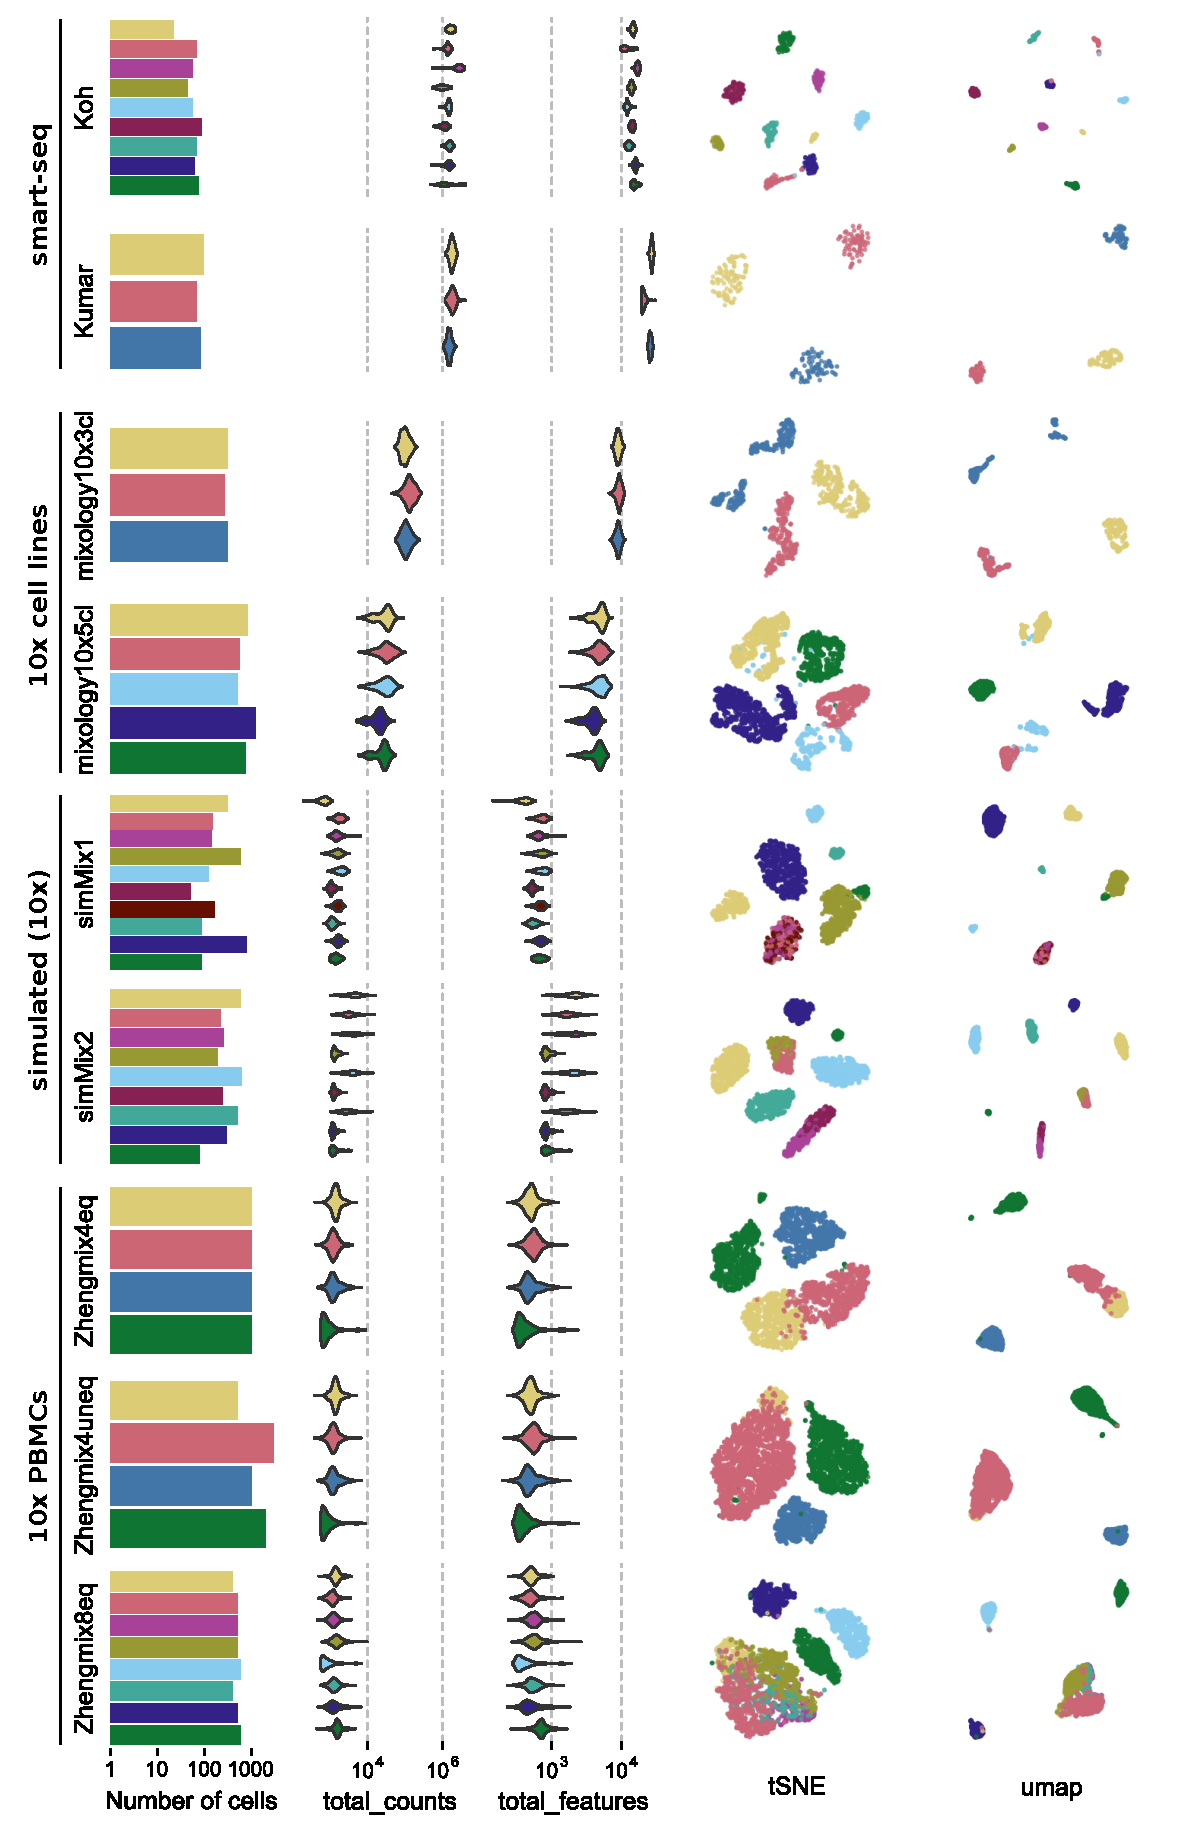
\includegraphics[width=\textwidth,keepaspectratio]{dataset_description}
    \caption{\textbf{Overview of the benchmark datasets used.}}
    \label{fig:figure1}
\end{figure}

\begin{figure}
    \centering
    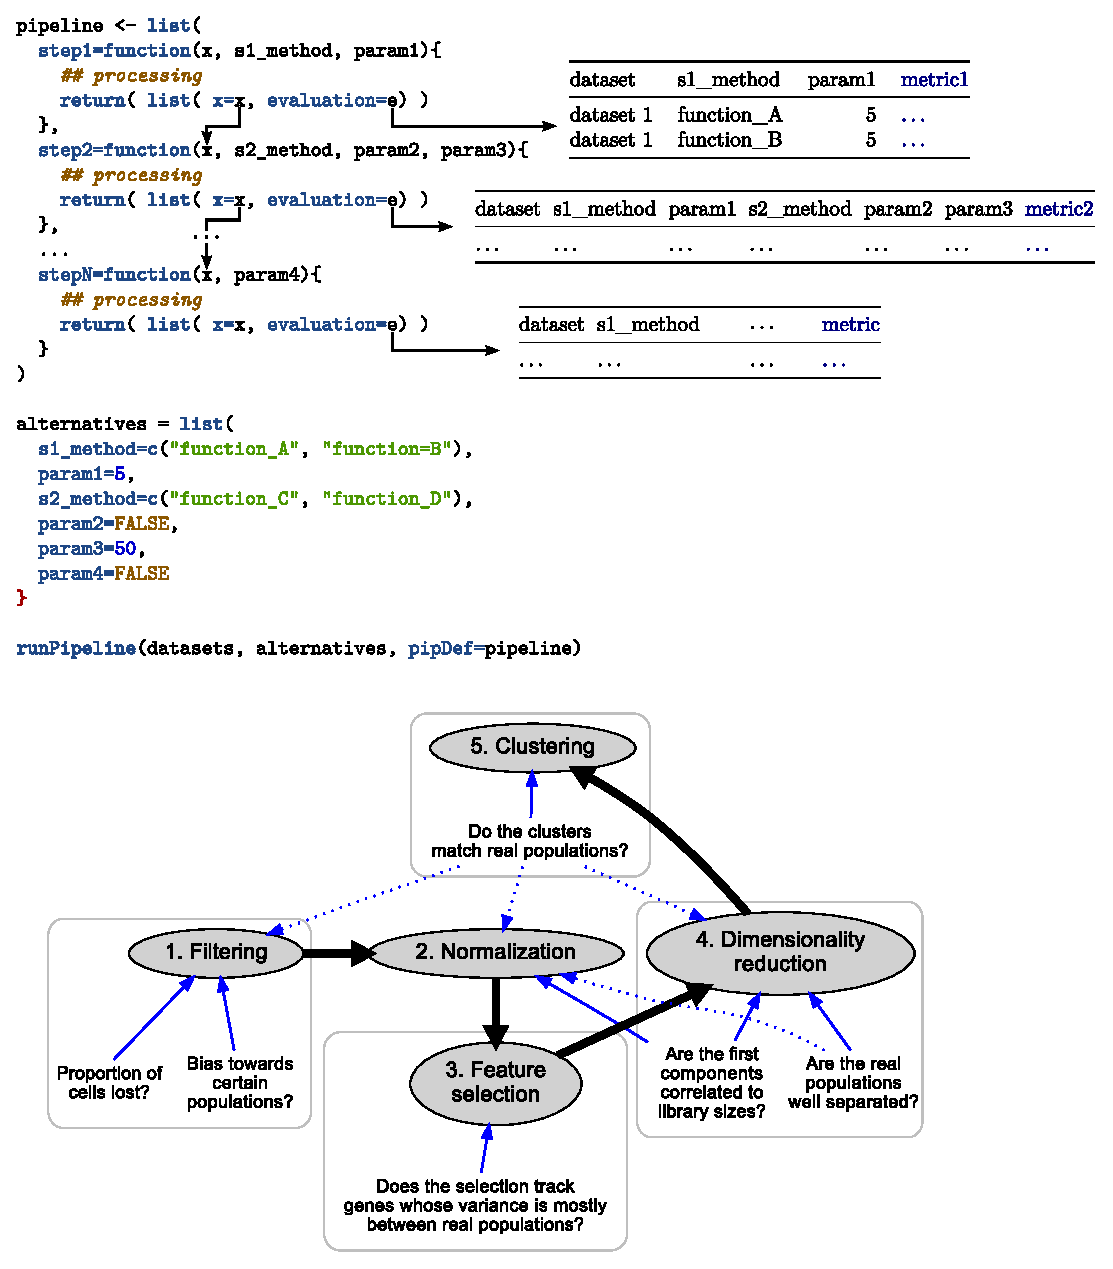
\includegraphics[width=\textwidth,keepaspectratio]{figure0}
    \caption{\textbf{Overview of the pipeComp framework and its application to a scRNAseq clustering pipeline.}}
    \label{fig:figure2}
\end{figure}

\subsection*{Filtering}

\subsubsection*{Doublet detection}

Doublets, defined as two cells sequenced under the same cellular barcode (for instance as a result of being captured in the same droplet), are fairly frequent in scRNAseq datasets, with estimates ranging from 1 to 10\% depending on the platform and cell concentration used \citep{bloomEstimating2018,kangMultiplexedDemuxlet2018}. While doublets of the same cell type are relatively innocuous for most downstream applications due to their conservation of the relative expression between genes, doublets formed from different cell types or states are likely to be misclassified and could potentially distort downstream analysis. In some cases, doublets can be identified through their unusually high number of reads and detected features, but this is not always the case (Supplementary Figure 2). A number of methods were developed to identify doublets, in most cases by comparing each cell to artificially-created doublets [REFs]. We therefore first evaluated the capacity of these methods to detect doublets using the two 10x datasets produced by \citep{tianMixology2018} with cells of different genetic identity, and for which therefore SNP information can be used as ground truth. We tested DoubletFinder [REF] and scran's doubletCells [REF], both of which use similarity to artificial doublets, and scds [REF], which relies on a combination of coexpression and binary classification. DoubletFinder integrates a thresholding based on the proportion of expected doublets, while scran and scds return scores which must be manually thresholded. In these cases, we ensured that the right number of cells would be called doublets.

In addition to these methods, we reasoned that an approach such as DoubletFinder could be considerably sped up by being applied directly on counts and by using a pre-clustering to create neotypic doublets (i.e. doublets from different cell types) more efficiently. We therefore developed a simple and fast package implementing this for doublet detection, with the added advantage of accounting for uncertainty in the expected doublet rate and using meta-cells from the clusters to even include triplets (see methods).

While most methods accurately identified the doublets in the 3 cell lines dataset (mixology10x3cl), the 5 lines dataset (mixology10x5cl) proved more difficult (Figure \ref{fig:figure3}B). Our method (scDblFinder) achieved the best accuracy while running in a very reasonable time (Figure \ref{fig:figure3}). Across datasets, cells called as doublets tended to be classified in the wrong cluster more often than other cells (Figure 1D). We therefore tested whether this method also improved the accuracy of the clustering across all benchmark datasets, and found that it consistently did (Figure \ref{fig:figure4}).

\begin{figure}
    \centering
    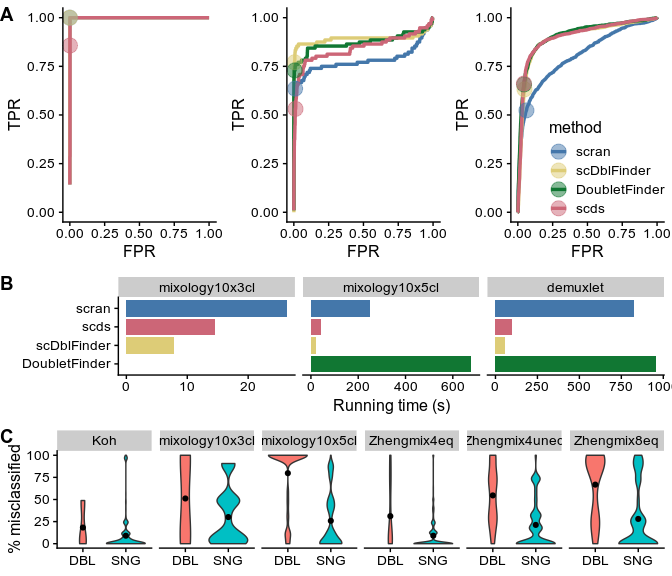
\includegraphics[width=\textwidth]{{main_figures/figure1_doublets_files/figure-html/figure1-1.png}}
    \caption{\textbf{Identification of doublet cells. A-B:} Receiver operating characteristic (ROC) curves of the tested doublet detection methods for the mixology10x3l (\textbf{A}) and mixology10x5cl (\textbf{B}) datasets. DoubletFinder failed due to an error on the mixology10x3cl dataset. \textbf{C:} Running time of the different methods. \textbf{D} Cell called as doublets by scDblFinder tend to be more often misclassified, i.e. assigned a wrong cluster. The corrected percentage of misclassification is the proportion of times a given cell is misclassified across hundreds of clustering pipelines with various parameters, minus the median misclassification rate of the cell's subpopulation.}
    \label{fig:figure3}
\end{figure}

\subsubsection*{Excluding more cells is not necessarily better}

Beyond doublets, a dataset might include low-quality cells whose elimination would reduce noise. This has for instance been demonstrated for cells that have a high content of mitochondrial reads, often as a result of cell degradation [REF]. A common practice is to exclude cells that differ considerably from most other cells on the basis of some such properties, for instance through the `isOutlier` function of `scater` which measures, for a given control property, the number of median absolute deviation of each cell from the mean of all cells. Supplementary Figure 1 shows the distributions of some of the typical cell properties commonly used. Of note, these properties tend to be correlated, but not always: for instance, while a high proportion of mitochondrial reads is often correlated with a high proportion of the counts in the top features, there can also be other reasons for an over-representation of highly-expressed features (Supplementary Figure 3). In addition, in our experience 10X datasets also exhibit a very tight correlation between the total counts and the total features even across very different cell types (Supplementary Figure 4). We therefore also measure the ratio between the two, and treat cells strongly departing from this trend with suspicion.

Reasoning that the cells we wish to eliminate are cells that would be misclassified, we measured the rate of misclassification of each cell in each dataset across a variety of clustering pipelines, correcting for the median misclassification rate of the subpopulation, and then evaluated what properties could be predictive of misclassification (Supplementary Figures 5-7). We could not identify any property or simple combination thereof that would be consistently predictive of misclassification; the only feature that consistently stood out across multiple datasets (the Zheng datasets) was that cells with a very high read counts have a higher chance of being misclassified.

We next investigated the impact of filtering according to various criteria on the accuracy of the clustering. We tested each aforementioned cell property, alone and in combinations, filtering above and/or below a certain threshold defined by different numbers of median absolute deviations. Reasoning that a bad cell would be bad in several distributions, we also included the optional rule that a cell should be excluded if it is an outlier in at least 2 or 3 distributions.

A first observation was that very stringent filtering (removing up to 20\% of the cells) was not generally associated with an increase in accuracy of the clustering (Supplementary Figure 8A). Moreover, stringent filtering tended to be biased towards the exclusion of specific subpopulations (Supplementary Figure 8B). Indeed, applying the same filtering criteria on individual clusters of cells (identified through scran's \textit{quickCluster} method) resulted in nearly no cell being filtered out, which suggests that filtering on the global population tends to discard cells of subpopulations with more extreme properties, rather than `bad` cells.

We next investigated the contribution of various criteria individually (Supplementary Figure 9). Interestingly, regression analysis suggests that increasing the number of distributions on which a cell must deviate in order to be excluded tended to be positively associated with ARI, while increasing the number of median absolute deviations required to be an outlier as associated with a decrease in ARI. We therefore suggest excluding cells that are outliers in more than 1 distribution. The impact of filtering on the basis of total counts or feature counts was not always robust, nor always positive, and we could detect no significant impact of filtering on the basis of the proportion of mitochondrial reads - however it must be said that the benchmark datasets count very few cells with a very high proportion of mitochondrial reads (Supplementary Figure 1). We therefore suggest to keep this criterion, but in a relatively lenient fashion, and not solely based on the median absolute deviation of the distribution. Filtering solely based on deviations from the distribution might be inadequate when the distribution is tight; in our experience, the proportion of mitochondrial counts in otherwise `healthy` cells can vary up to 8-12\% depending on the tissue. We therefore recommend using a combination of fixed and deviation based threshold, e.g. x $>$ 0.08 and x $>$ 2.5*MADs.

\begin{figure}
    \centering
    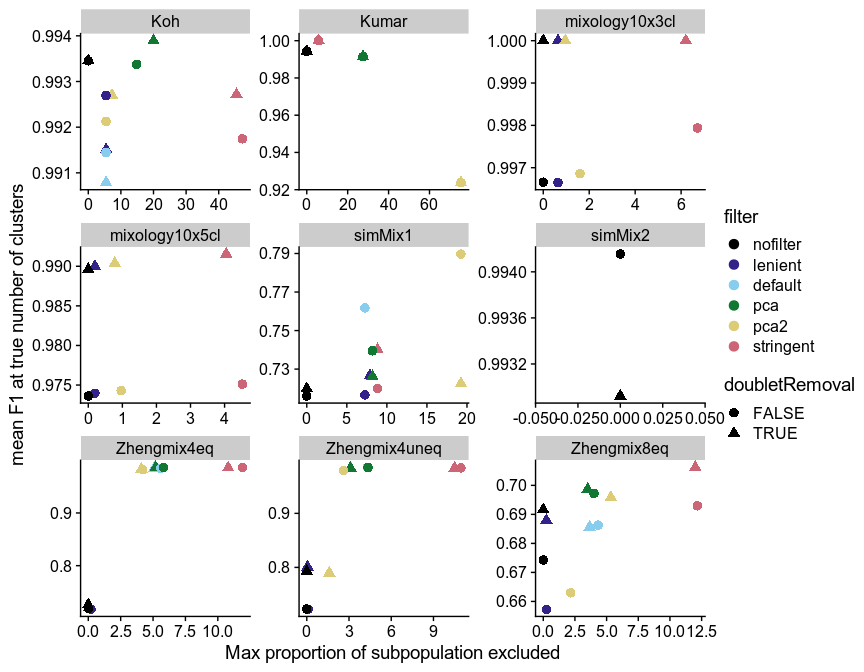
\includegraphics[width=\textwidth]{{main_figures/figure2_filtering_files/figure-html/figure2-1.png}}
    \caption{Proportion of cells filtered out and accuracy of the cluster (under two normalizations) for different sets of filters (see methods).}
    \label{fig:figure4}
\end{figure}

On the basis of these observations, we defined three sets of criteria as lenient, default and stringent filtering (see methods), and investigated them further. We found that filtering had a much milder impact than doublet removal (Figure \ref{fig:figure4}), and that more stringent filtering tended to result in higher silhouette width, in a higher proportion of the variance in the first components explained by subpopulations (Supplementary Figure 10), and often in a higher adjusted Rand index (ARI) of the clustering at the right number of clusters (Figure \ref{fig:figure4}). However, part of the gain is to be ascribed to the removal of cells from subpopulations (especially in the Zheng datasets) that are difficult to distinguish, and for which more stringent clustering did not improve silhouette width (Supplementary Figure 10A). For these reasons, we therefore recommend using a more lenient filter (e.g. lenient or default filter described here) or a cluster-based filter to avoid most of the subpopulation bias while excluding strong outliers.

\subsubsection*{Filtering features by type}

Mitochondrial reads have been associated with cell degradation, and it has been observed that much of scRNAseq clustering is determined by ribosomal genes [REF]. We therefore considered whether excluding one category of features or the other, or using only protein-coding genes, had impact on the ability to distinguish subpopulations (Supplementary Figure 11). Removal of ribosomal genes robustly reduced the quality of the clustering, suggesting that they represent real biological differences between subpopulations. Removing mitochondrial genes and restricting to protein-coding genes had a very mild impact.

\subsection*{Normalization and scaling}

We next investigated the impact of different normalization strategies. Beside the standard log-normalization included in Seurat, we tested scran's pooling-based normalization \citep{lunPooling2016}, sctransform's variance-stabilizing transformation \citep{hafemeisterSCtransform2019}, and normalization based on stable genes \citep{linStableGenes2018, deekeStablyExpressed2018}. 
In addition to log-normalization, the standard Seurat clustering pipeline scales features so that the PCA is not dominated by a small subset of the features, and we therefore included versions of the different normalization, with or without a subsequent scaling (except sctransform's variance-stabilizing transformation, given that, conceptually, it involves something analogous to scaling). 
Seurat's scaling function includes the option to regress out the effect of certain covariates, and we therefore tested its use with the proportion of mitochondrial counts and the number of detected features. Finally, it has been proposed that the use of stable genes, and in particular cytosolic ribosomal genes, can be used to normalize scRNAseq; we therefore evaluated a simple linear normalization based on the sum of these genes, as well as nuclear genes.

An important motivation of sctransform was the observation that, even after normalization, the first principal components of various datasets tended to correlate with library size, suggesting an inadequate normalization \citep{hafemeisterSCtransform2019}. We therefore first assessed to what extent the first principal component still retained a correlation with the library size and number of detected features, removing the confounding covariation with the subpopulation (Supplementary Figure 12A). The simple step of scaling tended to remove much of the correlation with these features, and in the absence of scaling, standard Seurat normalization resulted in fairly high correlation. sctransform had the lowest correlation, but most methods (including normalization based on stable genes) were able to remove most of the correlation when combined with scaling. The only exception is Seurat normalization with scaling regressing out the number of features, which surprisingly increased the correlation.

We next investigated the impact of normalization on the ability to distinguish subpopulations, which was much greater than that of filtering (Supplementary Figure 13). For many clusters, scaling tended to reduce both the average silhouette width (Supplementary Figure 12B) and the proportion of variance in the top principal components explained by subpopulations (Figure \ref{fig:figure5} and Supplementary Figure 13), and was associated with a poorer adjusted Rand index (ARI) of the resulting clustering (Figure \ref{fig:figure5}). Regressing out covariates systematically gave poorer performance on all metrics. sctransform produced the highest cluster average silhouette width (Supplementary Figure 12B) as well as ARI (Figure \ref{fig:figure5}), but not always the highest mean proportion of variance in the top components explained by subpopulations (Figure \ref{fig:figure5} and Supplementary Figure 13). Of note, even though sctransform is meant to be applied to data with unique molecular identifiers (UMI), it also performed fairly well with smartseq datasets. Interestingly, some clusters tended to be less well distinguished with sctransform than with non-scaled (and in some cases non-normalized) methods, suggesting that some procedures emphasize differences more useful to track some subpopulations than others, and hence the possibility that further developments in methods could improve this step.

\begin{figure}
    \centering
    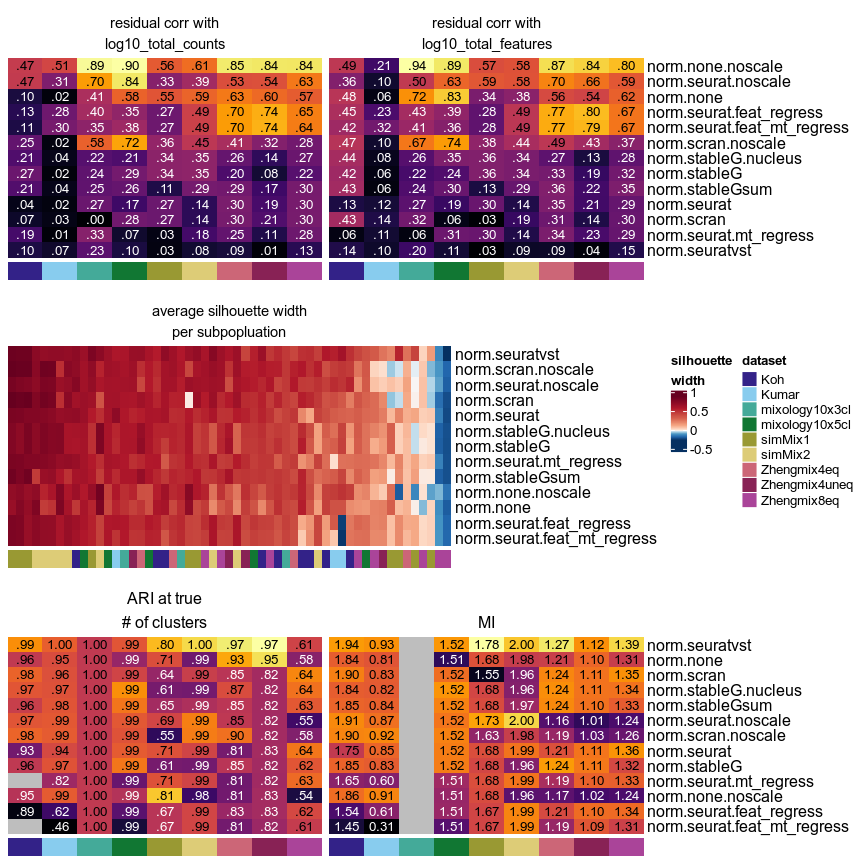
\includegraphics[width=\textwidth]{{main_figures/figure3_normalization_files/figure-html/figure3-1.png}}
    \caption{\textbf{Evaluation of normalization procedures:} proportion of the variance in the first 5 components explained by the subpopulations, median ARI, and ARI at the true number of clusters.}
    \label{fig:figure5}
\end{figure}

Finally, although there were differences in specific cases, we observed no robust tendency of certain normalization methods towards over- or under-estimating the number of clusters when using with Seurat clustering (Supplementary Figure 14).

\subsection*{Feature selection}

A standard clustering pipeline typically involves a step of selecting highly-variable genes, which is complicated by the digital nature and the mean-variance relationship of RNAseq. Seurat's earlier approaches involved the use of dispersion estimates standardized for the mean expression levels, while more recent versions rely of a different measure of variance, again standardized. Of note, while adjusting for the mean-variance relationship removes much of the bias towards highly-expressed genes, it is plausible that this bias reflects biological relevance and hence is actually helpful in classifying cell types. Another common practice for selecting features is to use those with the highest mean expression, and recently \citep{townesGlmpca2019} instead suggested to use deviance, while sctransform provides its own ordering the genes by transformed variance. We therefore compared these methods.

Reasoning that a selection method should ideally select genes whose variability is more between subpopulations than within, we first assessed whether each selection method selected genes with a high proportion of variance or deviance explained by (real) subpopulations (the latter estimated through edgeR). Estimates of variance explained by subpopulations based on a standard Seurat normalization or on sctransform data were highly correlated (Supplementary Figure 14A), and there was also a good agreement with deviance explained, although lowly-expressed genes in particular could have a high deviance explained without having much of their variance explained by subpopulations (Supplementary Figure 15B-D). We therefore compared, using both of these estimates, the proportion of the cumulative variance/deviance explained by the top X genes that could be retrieved by each gene ranking method (Supplementary Figures 16-17). We first focused on the first 1000 genes to highlight differences between methods, although the differences tended to decrease with a higher number of genes selected (Figure \ref{fig:figure6}A). A first observation was that standardized measures of variability were systematically worse than their non-standardized  counterparts in selecting genes with a high proportion of variance explained by subpopulations, while instead proving most of the time superior in selecting genes with a high deviance explained by subpopulations (Figure \ref{fig:figure6} and Supplementary Figures 16-17). Deviance proved the method of choice to maximize the former (with mere expression level proving surprisingly good), but did not perform so well to select genes with a high deviance explained.

\begin{figure}
    \centering
    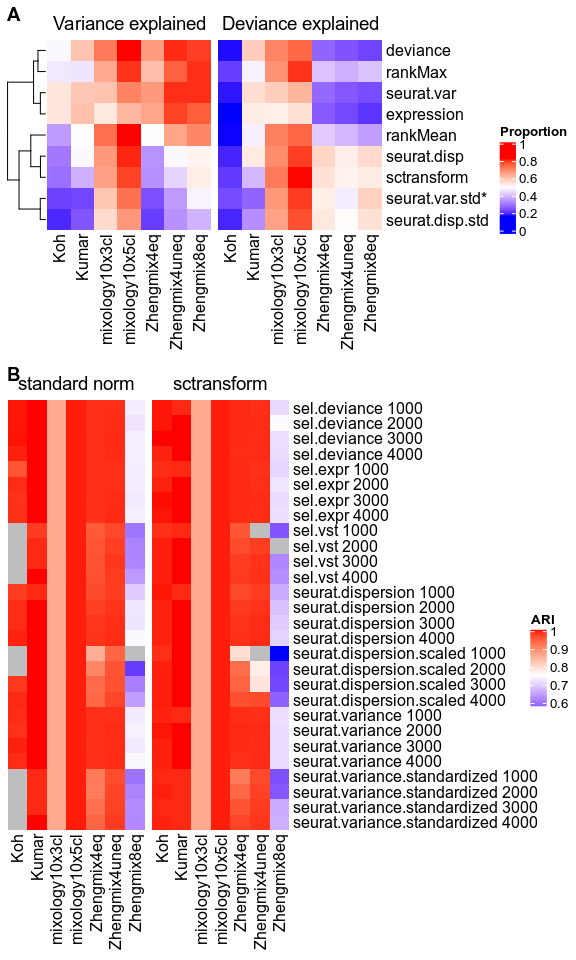
\includegraphics[scale=0.6]{{main_figures/figure4_selection_files/figure-html/figure4-1.png}}
    \caption{\textbf{Evaluation of feature selection methods. A:} Ability of different feature ranking methods to capture genes with a high proportion of variance (left) or deviance (right) explained by real subpopulations. rankMean and rankMax refer to, respectively, the mean rank and the maximum rank in the following metrics: variance, standardized variance, sctransform, deviance. \texbf{B:} Accuracy of clustering (at the right number of clusters) based on the given selection methods and number of genes selected.}
    \label{fig:figure6}
\end{figure}

We next investigated whether a selection based on these methods impacted the proportion of variance explained by subpopulations in the first principal components (Supplementary Figure 18). To validate the previous assay, included a selection based on the genes whose proportion variance or deviance explained was highest. Interestingly, while these selections were on average the top-ranking methods, they were not systematically so for all dataset.

The main observations were reflected in the ARI of the resulting clustering (Figure 4B): non-standardized measures of variability, including mere expression level, tended to outperform more complex metrics. In general, we found deviance and Seurat's un-standardized estimate of variance to provide the best results across datasets and normalization methods. Increasing the number of features selected also systematically led to an increase in the accuracy of the clustering.

\subsection*{Dimensionality reduction}

We next investigated the step of dimensionality reduction, comparing in particular Seurat's PCA, GLM-PCA \citep{townesGlmpca2019}, and a two-step PCA procedure in which cells are first clustered in rough clusters according to a standard PCA, a new PCA is performed on each, and the main components of the two are put together (see methods). Seurat's default PCA weighs the cell embeddings by the variance of each component, so we also tested the impact of this weighting with each method.

The impact of the dimensionality reduction method was far greater than that of normalization or feature selection (e.g. Supplementary Figure 19). Although the first components identified by GLM-PCA tended to have a higher proportion of their variance explained by real subpopulations and increase the average silhouette width of already well-defined subpopulations, overall Seurat's PCA procedure proved superior on all metrics (Figure \ref{fig:figure7} and Supplementary Figures 19-21). 
In particular, weighing the components had a strong positive impact on silhouette widths and resulting ARI.

\begin{figure}
    \centering
    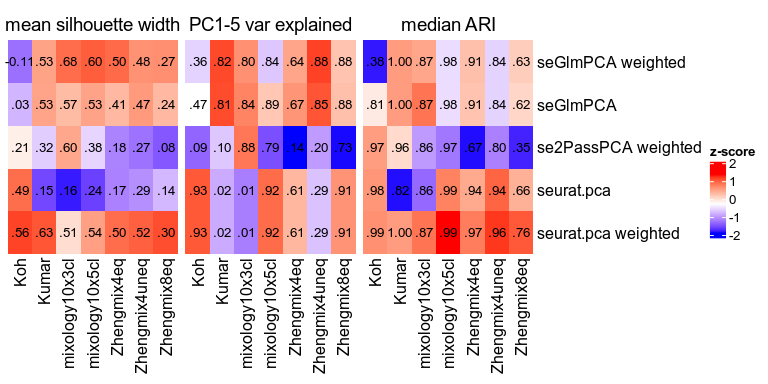
\includegraphics[width=\textwidth]{{main_figures/figure5_dr_files/figure-html/unnamed-chunk-2-1.png}}
    \caption{Evaluation of the dimensionality reduction strategies.}
    \label{fig:figure7}
\end{figure}

We next investigated the impact of the number of dimensions used on the clustering. Overall, increasing the number of dimensions robustly led to a decrease in the number of clusters, although the effect was milder with data processed through sctransform (Supplementary Figures 14 and 22). This tended to be translated to the accuracy of the clustering (Supplementary Figure 23), although in both cases (number of clusters and ARI) the resolution parameter had a much stronger impact.

\subsubsection*{Rules for selecting components}

\subsection*{Clustering}



\section*{Discussion}

For research articles this section should discuss the implications of the findings in context of existing research and highlight limitations of the study. For study protocols and methodology manuscripts this section should include a discussion of any practical or operational issues involved in performing the study and any issues not covered in other sections.

\section*{Conclusions}

This should state clearly the main conclusions and provide an explanation of the importance and relevance of the study to the field.

\section*{Methods}

\subsection*{Code and data availability}

All analyses were performed through the \href{pipComp}{https://github.com/plger/pipComp} R package, which implements the pipeline framework described here. All code to reproduce each figure is available in the \url{https://github.com/markrobinsonuzh/scRNA\_pipelines\_paper} repository, which also includes the basic datasets with a standardized annotation.

The gene counts for the two mixology datasets were downloaded from the  \href[CellBench repository]{https://github.com/LuyiTian/CellBench\_data/data/sincell\_with\_class.RData}, commit 74fe79e. For the other datasets, we used the unfiltered counts from \citep{duoClustering2018}, available on the corresponding repository \url{https://github.com/markrobinsonuzh/scRNAseq\_clustering\_comparison}. For simplicity, all starting \textit{SingleCellExperiment} objects with standardized metadata are available on \url{https://github.com/markrobinsonuzh/scRNA\_pipelines\_paper}.

\subsection*{Software and package versions}
Analyses were performed in R 3.6.0 (bioconductor 3.9), and the following packages were installed from github repositories: Seurat (version 3.0.0), sctransform (0.2.0), DoubletFinder (2.0.1), scds (1.0.0), pipComp (0.2). The code for the glmPCA was obtained from \url{https://github.com/willtownes/scrna2019} (commit 1ddcc30ebb95d083a685f12fe81d35dd1b0cb1b2).

\subsection*{Default pipeline parameters}
(to come)

\subsection*{Doublet detection method}
Our doublet detection method is available at \url{https://github.com/plger/scDblFinder}. Version 0.1 was used here. Briefly, we first cluster the cells using scran's \textit{quickCluster} method, favouring overclustering (default minimum size of 20), and reduce the dataset to the union of 1500 most expressed genes of each cluster. We then create 75\% of the artifical doublets by sampling the two cells specifically from different clusters, and 25\% by entirely random sampling (in case the clustering was erroneous), and summing the counts of each pair of cells. We also create meta-cells from each cluster, and use them to create additional doublets and triplets. We then combine them with the real cells, convert the counts to scaled column ranks, and build a graph of the \textit{k} (default 10) nearest neighbors using scran. We then calculate, for each cell, the proportion of its neighbors that are artificial doublets. This ratio serves as a doublet score, which is then thresholded by simultaneously minimizing the error in classifying real vs artificial doublets and the deviation from the distribution of expected doublet rate (accounting for homotypic doublets as done by DoubletFinder). For the pipeline comparison here, the expected doublet rate was set to 2.1\% (with a 1\% standard deviation) on the basis of the mixology datasets.

\subsection*{Filter sets}
The \textit{default} set of filters excludes cells that are outliers according to at least two of the following thresholds: log10\_total\_counts $>$2.5 MADs or $<$5 MADs, log10\_total\_features $>$2.5 MADs or $<$5 MADs, pct\_counts\_in\_top\_20\_features $>$ or $<$ 5 MADs, featcount\_dist (distance to expected ratio of log10 counts and features) $>$ or $<$ 5 MADs, pct\_counts\_Mt $>$ 2.5 MADs and $>$ 0.08.

The \textit{stringent} set of filters uses the same thresholds, but excludes a cell if it is an outlier on any single distribution. 

The \textit{lenient} set of filters excludes cells that are outliers on at least two distributions by at least 5 MADs, except for pct\_counts\_Mt where the threshold is $>$ 3 MADs and $>$ 0.08.

For cluster-wise filters, clusters were first identified with \textit{scran::quickCluster} and the filters were then applied separately for each cluster.


\subsection*{Variance and deviance explained}

Unless specified otherwise, the variance in gene expression explained by subpopulations was calculated on the data normalized and transformed through sctransform. For each gene, we fitted a linear model using the subpopulation as only independent variable (\textasciitilde subpopulation), and used the R-squared as a measure of the variance explained. The same method was used for principal components.

The deviance explained by subpopulations was calculated directly on counts using the \textit{pipComp::getDevianceExplained} function. The function uses edgeR to fit two models, a full \textasciitilde librarySize+subpopulation model and a reduced \textasciitilde librarySize model. For each gene, the deviance explained is then the difference between the deviance of each models, divided by the deviance of the reduced model. In the rare cases where this resulted in a negative deviance explained, it was set to zero.

To estimate the correlation between the principal components and covariates such as library size, we first fitted a linear model on the subpopulations, and correlated the residuals of this model with the covariate of interest.


%%%%%%%%%%%%%%%%%%%%%%%%%%%%%%%%%%%%%%%%%%%%%%
%%                                          %%
%% Backmatter begins here                   %%
%%                                          %%
%%%%%%%%%%%%%%%%%%%%%%%%%%%%%%%%%%%%%%%%%%%%%%

\begin{backmatter}

\section*{Competing interests}
  The authors declare that they have no competing interests.

\section*{Author's contributions}
    Text for this section \ldots

\section*{Acknowledgements}
  Text for this section \ldots
%%%%%%%%%%%%%%%%%%%%%%%%%%%%%%%%%%%%%%%%%%%%%%%%%%%%%%%%%%%%%
%%                  The Bibliography                       %%
%%                                                         %%
%%  Bmc_mathpys.bst  will be used to                       %%
%%  create a .BBL file for submission.                     %%
%%  After submission of the .TEX file,                     %%
%%  you will be prompted to submit your .BBL file.         %%
%%                                                         %%
%%                                                         %%
%%  Note that the displayed Bibliography will not          %%
%%  necessarily be rendered by Latex exactly as specified  %%
%%  in the online Instructions for Authors.                %%
%%                                                         %%
%%%%%%%%%%%%%%%%%%%%%%%%%%%%%%%%%%%%%%%%%%%%%%%%%%%%%%%%%%%%%

% if your bibliography is in bibtex format, use those commands:
\bibliographystyle{bmc-mathphys} % Style BST file (bmc-mathphys, vancouver, spbasic).
\bibliography{bmc_article}      % Bibliography file (usually '*.bib' )
% for author-year bibliography (bmc-mathphys or spbasic)
% a) write to bib file (bmc-mathphys only)
% @settings{label, options="nameyear"}
% b) uncomment next line
%\nocite{label}

% or include bibliography directly:
% \begin{thebibliography}
% \bibitem{b1}
% \end{thebibliography}

%%%%%%%%%%%%%%%%%%%%%%%%%%%%%%%%%%%
%%                               %%
%% Figures                       %%
%%                               %%
%% NB: this is for captions and  %%
%% Titles. All graphics must be  %%
%% submitted separately and NOT  %%
%% included in the Tex document  %%
%%                               %%
%%%%%%%%%%%%%%%%%%%%%%%%%%%%%%%%%%%

%%
%% Do not use \listoffigures as most will included as separate files

\section*{Figures}
  \begin{figure}[h!]
  \caption{\csentence{Sample figure title.}
      A short description of the figure content
      should go here.}
      \end{figure}

\begin{figure}[h!]
  \caption{\csentence{Sample figure title.}
      Figure legend text.}
      \end{figure}

%%%%%%%%%%%%%%%%%%%%%%%%%%%%%%%%%%%
%%                               %%
%% Tables                        %%
%%                               %%
%%%%%%%%%%%%%%%%%%%%%%%%%%%%%%%%%%%

%% Use of \listoftables is discouraged.
%%
\section*{Tables}

\begin{table}[h!]
\caption{Overview of the benchmark datasets}
\label{tab:table1}
\begin{tabular}{rlrrl}
  \hline
dataset & source & protocol & nbCells & subpops & description \\ 
  \hline
Koh & GSE85066 & SMARTer & 531 &   9 & FACS purified H7 hESC in different differention stages \\ 
  Kumar & GSE60749 & SMARTer & 246 &   3 & Mouse ESC cultured in different conditions \\ 
  Zhengmix4eq & \citep{duoClustering2018} & 10x & 3994 &   4 & Mixtures of FACS purified PBMCs \\ 
  Zhengmix4uneq & \citep{duoClustering2018} & 10x & 6498 &   4 & Mixtures of FACS purified PBMCs \\ 
  Zhengmix8eq & \citep{duoClustering2018} & 10x & 3994 &   8 & Mixtures of FACS purified PBMCs \\ 
  mixology10x3cl & \cite{tianMixology2018} & 10x & 902 &   3 & Mixture of 3  cancer cell lines from CellBench \\ 
  mixology10x5cl & \cite{tianMixology2018} & 10x & 3918 &   5 & Mixture of 5 cancer cell lines from CellBench \\ 
   \hline
\end{tabular}
\end{table}

%%%%%%%%%%%%%%%%%%%%%%%%%%%%%%%%%%%
%%                               %%
%% Additional Files              %%
%%                               %%
%%%%%%%%%%%%%%%%%%%%%%%%%%%%%%%%%%%

\section*{Additional Files}
  \subsection*{Additional file 1 --- Sample additional file title}
    Additional file descriptions text (including details of how to
    view the file, if it is in a non-standard format or the file extension).  This might
    refer to a multi-page table or a figure.

  \subsection*{Additional file 2 --- Sample additional file title}
    Additional file descriptions text.


\end{backmatter}
\end{document}
